\subsection{Expected signal}
In order to estimate rates, resolution and acceptance due to the
Primakoff reaction on lead, $\gamma ^{208}\rm{Pb}\rightarrow \pi^0
\pi^0\, \rm{Pb}$, we take the reaction process to be the same as for
charged pion production and given in Eq.~8 of the Proposal for the
Charged Pion Polarizability experiment \cite{CPPexp}, which is
reproduced here for convenience:
\begin{eqnarray}
\frac{d^2\sigma}{d\Omega_{\pi\pi}dW_{\pi\pi}} = \frac{2\alpha Z^2}{\pi^2} \frac{E^4_\gamma \beta^2}{W_{\pi\pi}} \frac{\sin^2\theta_{\pi\pi}}{Q^4} |F(Q^2)|^2 \sigma(\gamma\gamma\rightarrow\pi^0\pi^0) (1+P_\gamma \cos{2\phi_{\pi\pi}}).   \label{eq:PrimakoffSignal}
\end{eqnarray}
The $\gamma\gamma$ cross section for charged pions has been
substituted with the cross section for neutral pions, namely
$\sigma(\gamma\gamma\rightarrow\pi^0\pi^0)$. In this expression,
$\Omega_{\pi\pi}$ is the solid angle in the laboratory frame for the
emission of the $\pi\pi$ system, $W_{\pi\pi}$ is the $\pi\pi$
invariant mass, Z is the atomic number of the target, $\beta$ is the
velocity of the $\pi\pi$ system, $E_\gamma$ is the energy of the
incident photon, $F(Q^2)$ is the electromagnetic form factor for the
target with final-state-interaction (FSI) corrections applied,
$\theta_{\pi\pi}$ is the lab angle for the $\pi\pi$ system,
$\phi_{\pi\pi}$ is the azimuthal angle of the $\pi\pi$ system relative
to the incident photon polarization, and $P_\gamma$ is the incident
photon polarization.\footnote{The expression for the cross section in
  terms of invariant quantities can be found in
  Ref.\,\cite{hdnote3186}.}
\begin{figure}[tph]
\centering
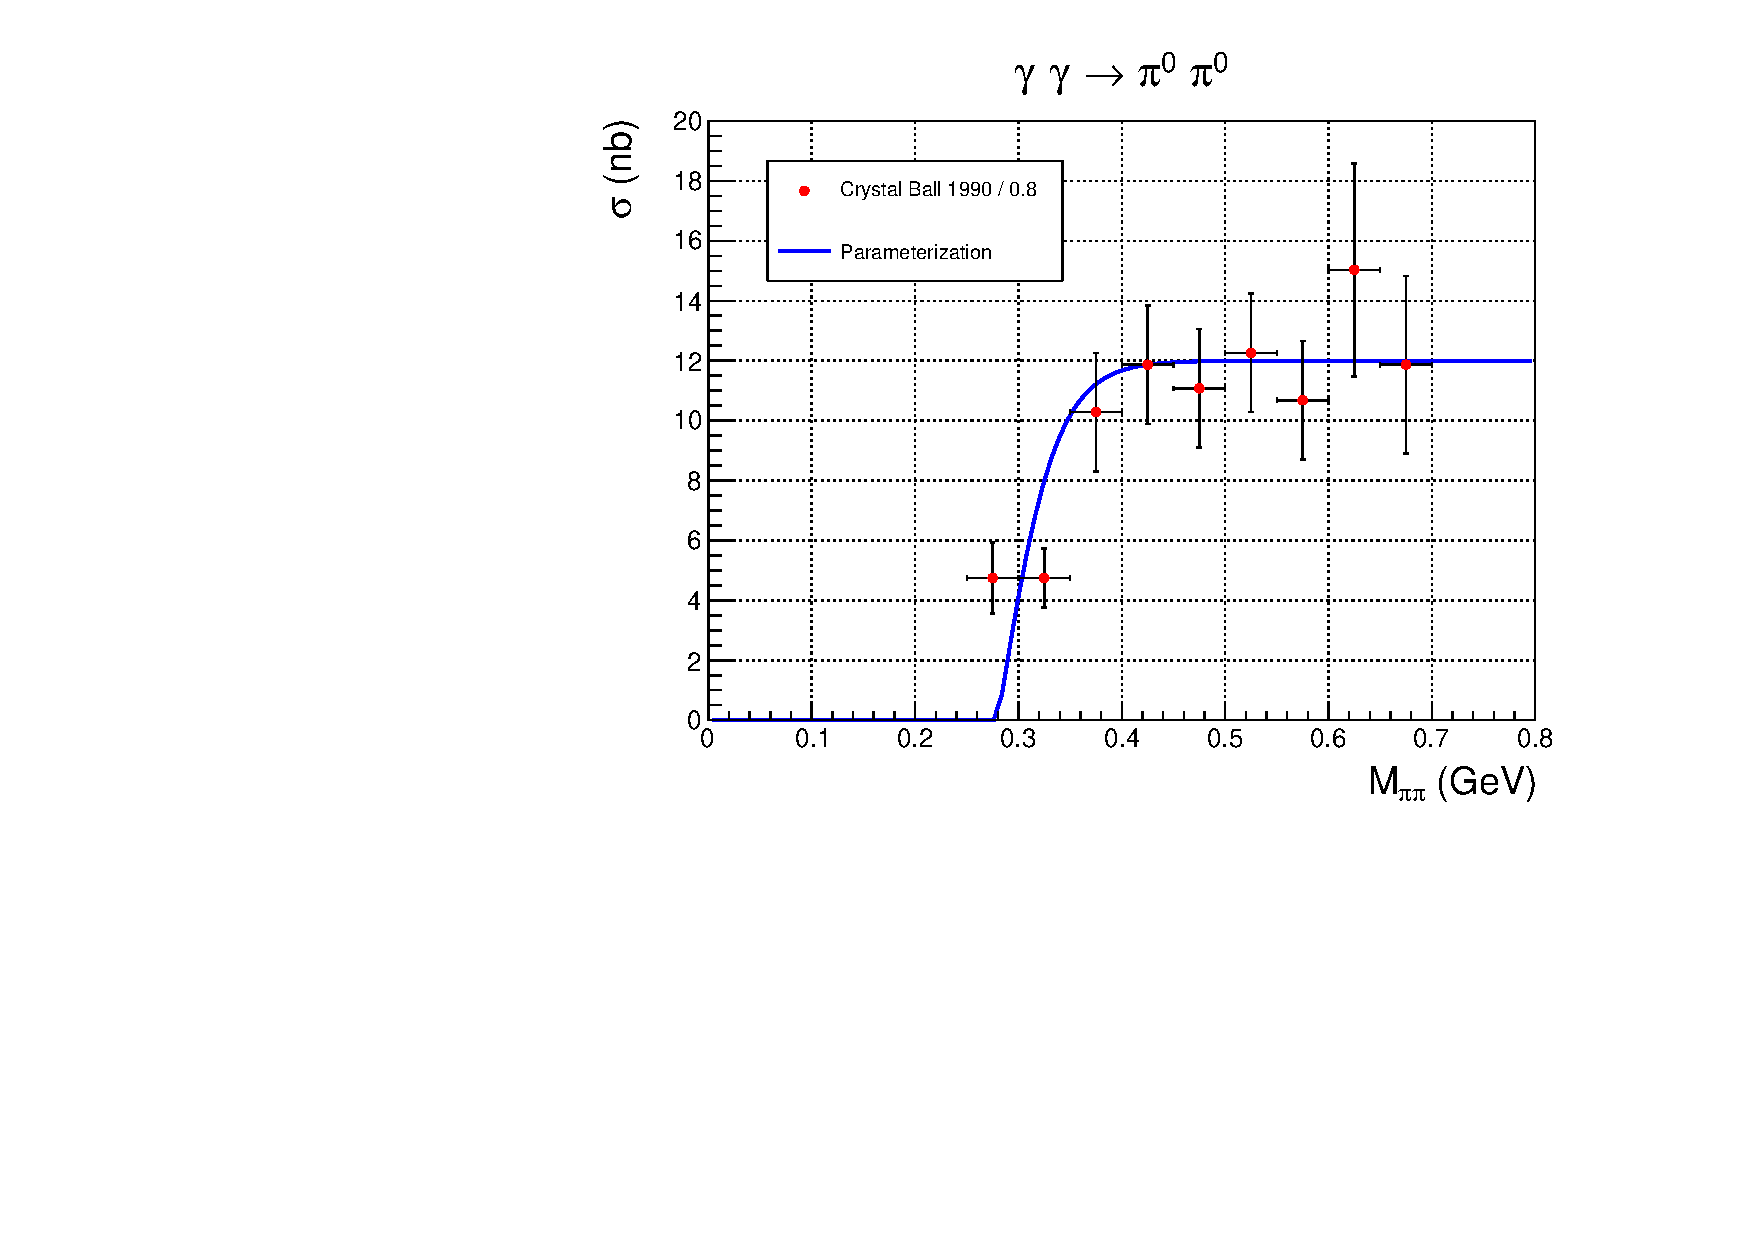
\includegraphics[page=1,width=4.75in]{figures/sigma_2pi0_figs.pdf}
\caption{Parameterization of the $\sigma(\gamma\gamma\rightarrow \pi^0\pi^0)$ cross section as a function
of the 2$\pi$ invariant mass compared to the data from Crystal Ball \cite{Marsiske:1990hx}.
\label{fig:sigma_2pi0_figs_1}}
\end{figure}

The cross section for $\sigma(\gamma\gamma\rightarrow\pi^0\pi^0)$ has
been measured by the Crystal Ball Collaboration
\cite{Marsiske:1990hx}, albeit with limited statistical precision. We
have parameterized the cross section for $W_{\pi\pi}<0.8$ GeV, which
is of specific interest to this program as shown in
Fig.~\ref{fig:sigma_2pi0_figs_1}. Using this parameterization and
Eq.~\ref{eq:PrimakoffSignal}, we can calculate the photoproduction
cross section on lead, which is shown in
Fig.~\ref{fig:sigma_2pi0_figs_2}.
\begin{figure}[tph]
\centering
\includegraphics[page=2,width=4.75in]{figures/sigma_2pi0_figs.pdf}
\caption{Primakoff cross section for $\gamma Pb \rightarrow Pb\, \pi^0 \pi^0$ using the parameterization of  $\sigma(\gamma\gamma\rightarrow \pi^0\pi^0)$ in the previous figure. The integrated cross section is 0.3\,$\mu$b/nucleus.
\label{fig:sigma_2pi0_figs_2}}
\end{figure}
The integrated cross section is $0.30 \pm 0.05~\mu$b/nucleus. The
uncertainty comes from the model dependence and was obtained by
comparing two different calculations using completely different
parameterizations for the nuclear form factor on lead, $F(Q^2)$. For
reference,
we note that the cross section for charged pions $(\pi^+\pi^-$)
production is 10.9\,$\mu$b, a factor of 30 larger.

The number of neutral-pion-Primakoff-signal events produced during 20
PAC days is shown in Fig.~\ref{fig:sigma_2pi0_figs_3}. The impacts of
detector trigger, acceptance and resolution are discussed in the next
section.
\begin{figure}[tph]
\centering
\includegraphics[page=3,width=4.75in]{figures/sigma_2pi0_figs.pdf}
\caption{Estimated production rate  for $\gamma \rm{Pb}\rightarrow \pi^0\pi^0\,\rm{Pb}$ as a function 2$\pi$ mass. For this calculation, it is assumed the detector has perfect resolution and has a linearly increasing efficiency from zero at threshold up to 0.4 at 0.34 GeV (see top right of Fig.\,\ref{fig:twopi_primakoff_DSelect_p1_W_100000_sum} ).
\label{fig:sigma_2pi0_figs_3}}
\end{figure}

\subsection{Detector resolution}
\label{sec:acceptance}
The response of the GlueX detector to neutral pion Primakoff events
was simulated using the standard GlueX generation and reconstruction
tools, but with the specific geometry for the CPP experiment. The schematic of the detector configuration is shown in
Fig.~\ref{fig:GlueX_cpp}. The primary differences between the
standard GlueX geometry and CPP are summarized in
Table\,\ref{tab:ccp_config}. For this experiment, the main differences
include a) coherent peak position at 5.5-6 GeV and re-positioning of
the microscope to cover the coherent peak, b) solid $^{208}$Pb at
z=1cm, and c) Start counter removed. For the CPP experiment, the
addition of muon identification chambers behind the FCAL is
critical. However, for neutral pions this addition plays no role
because the photons are detected in the FCAL. The GEANT4 simulation,\footnote{The initial simulations used GEANT3
and show similar results.}
which is used for these studies, includes most changes except for the
addition of the muon chambers, which are not needed. In addition, the
microscope geometry has not been modified and we use the tagger
hodoscope for the region of interest in the simulation. The slightly reduced
energy of the hodoscope relative to the microscope has little impact
and the gaps between counters are ignored when simulating the tagged
flux.
\begin{figure}[h!]
\centering
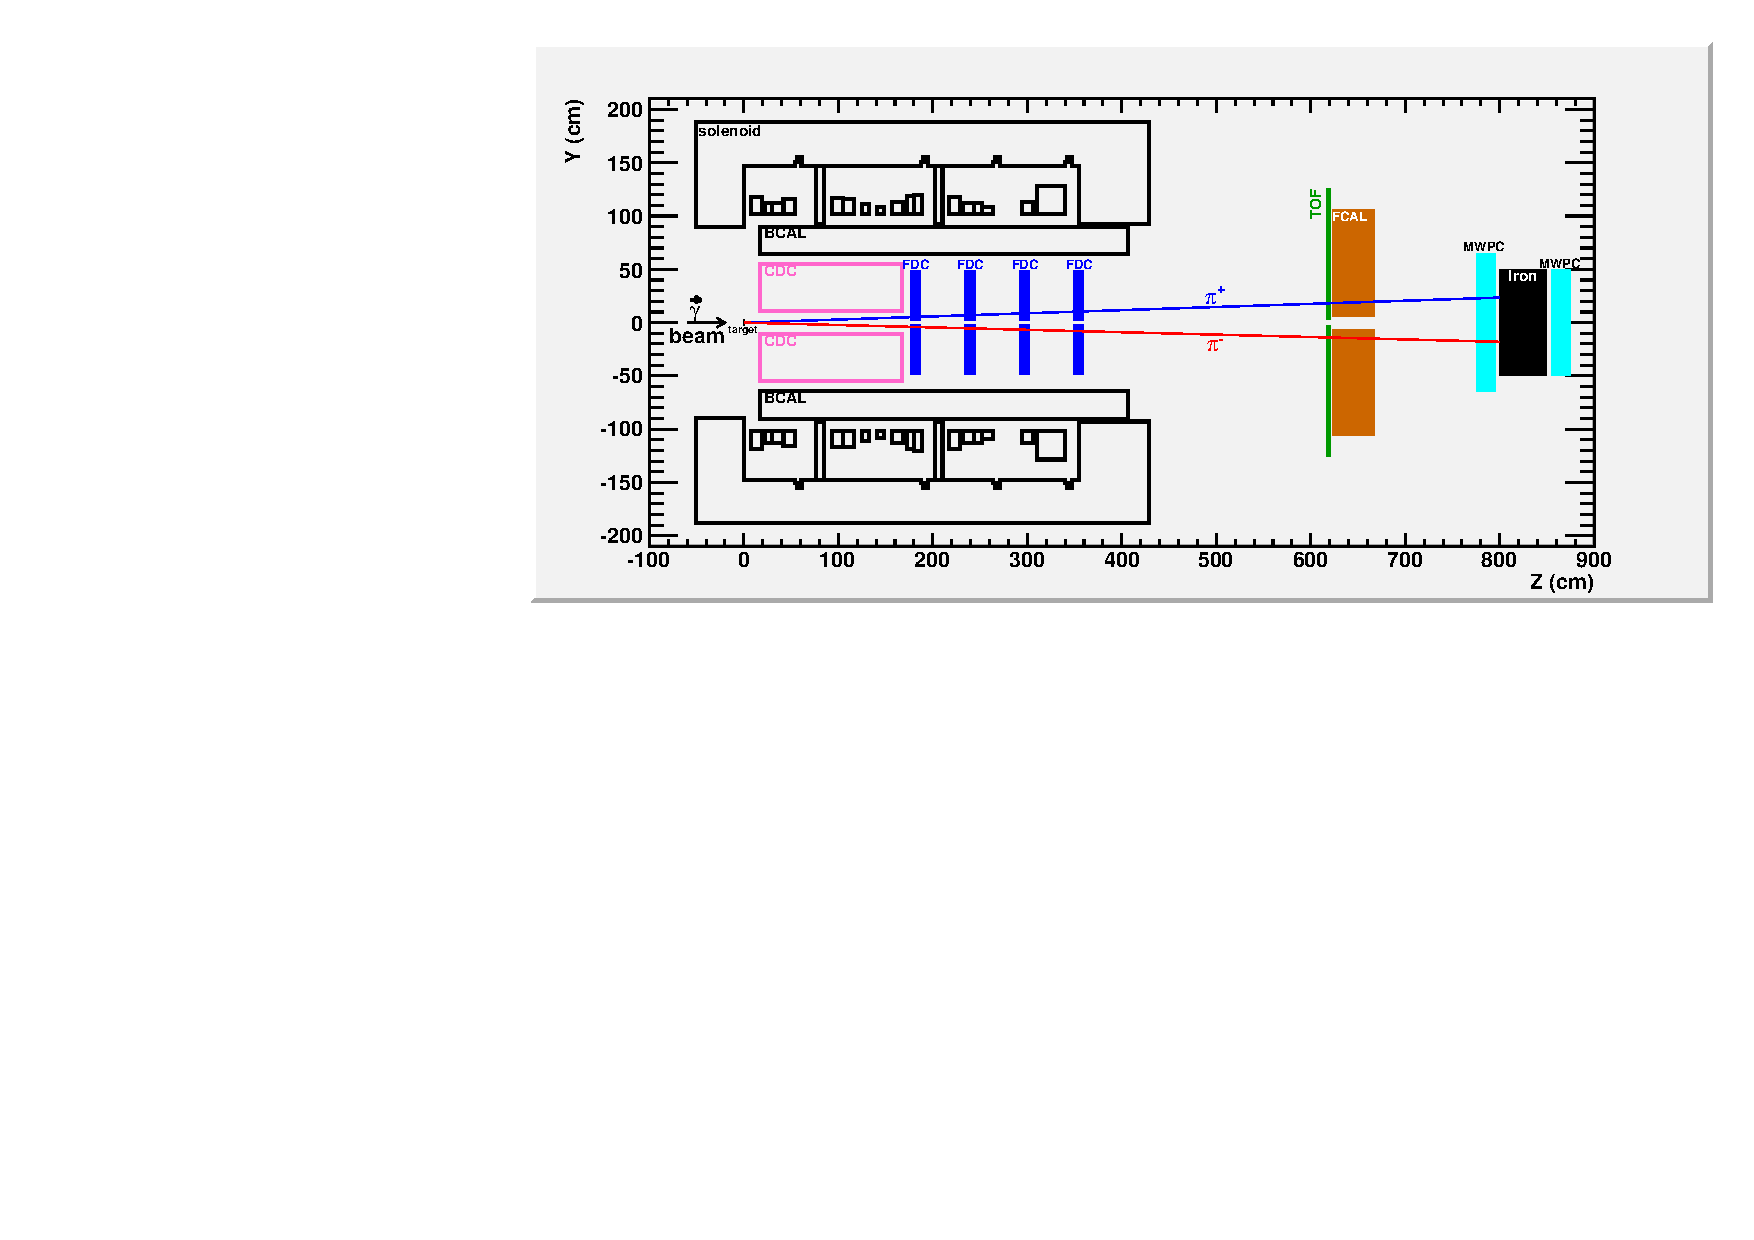
\includegraphics[width=5.25in]{figures/GlueX_cpp.pdf}
\caption{Diagram of the GlueX detector including the additional muon chambers for the CPP experiment.}
\label{fig:GlueX_cpp}
\end{figure}

The Primakoff signal was generated according to the cross section
described in the previous chapter, using the
\emph{gen\_2pi0\_primakoff} program, which is a modified version of the CPP event generator. By default, the production amplitudes are
symmetrized between the two identical $\pi^0$'s by AmpTools. One
hundred thousand events of Primakoff and nuclear coherent interactions 
(see Section\,\ref{sec:NCback}) were generated with $M_{\pi\pi}<$0.9 GeV.
We used random triggers from run 30401\footnote{Run 30401 is a low-intensity run for GlueX,
but represents considerably higher background than expected for this experiment.} to add tagger accidentals 
and random hits in the drift chambers. These events were fed to GEANT4 to track particles, and subsequently
processed using \emph{mcsmear} to simulate the detector response. The
simulated events were then analyzed using the GlueX event filter to
analyze the reaction $\gamma Pb \rightarrow \pi^0 \pi^0$ with a
missing Pb nucleus and to constrain the detected photon pairs to the
$\pi^0$ mass. Energy and momentum conservation is imposed on the reaction as well as the requirement that all photons originate from a common vertex. The output of the reconstruction, both kinematically
fit and ``measured" quantities, were available for inspection.

In the following we show various reconstructed quantities as well as
estimated resolutions. The distribution of generated photon energy and
the unconstrained reconstructed momenta of the two pions are shown in
Fig.~\ref{fig:EgP1P2_signal_DSelector}.
\begin{figure}[tph]
\centering
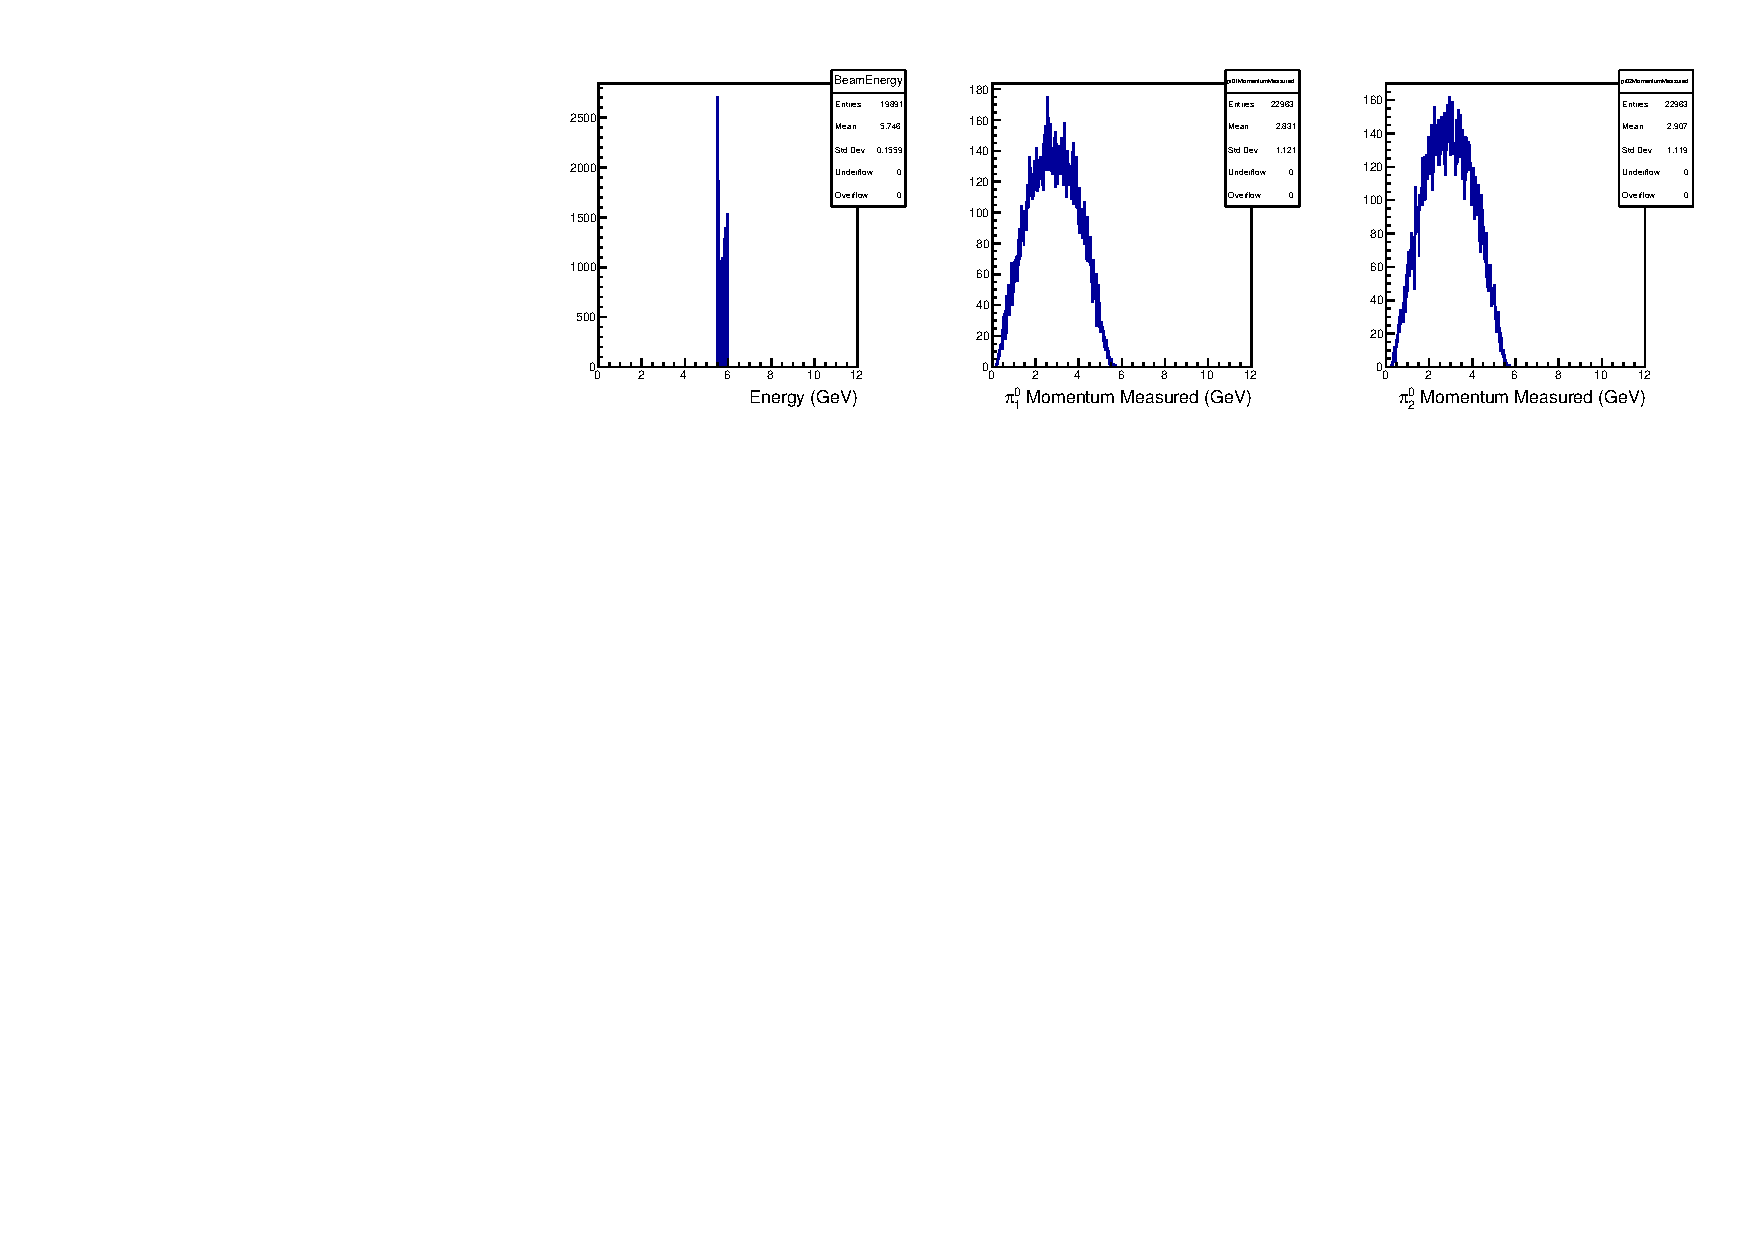
\includegraphics[width=6in]{figures/EgP1P2_signal_DSelector.pdf}
\caption{Left: Generated photon energies. The increased rate near 5.5 GeV is due to tagger accidentals. Center: Reconstructed momentum distribution of one $\pi^0$. Right: Reconstructed momentum distribution of the second $\pi^0$.
\label{fig:EgP1P2_signal_DSelector}}
\end{figure}
The missing mass, 2$\pi$ mass and $-t$ distributions are shown in Fig.~\ref{fig:MMMpipit_signal_DSelector}.
\begin{figure}[tph]
\centering
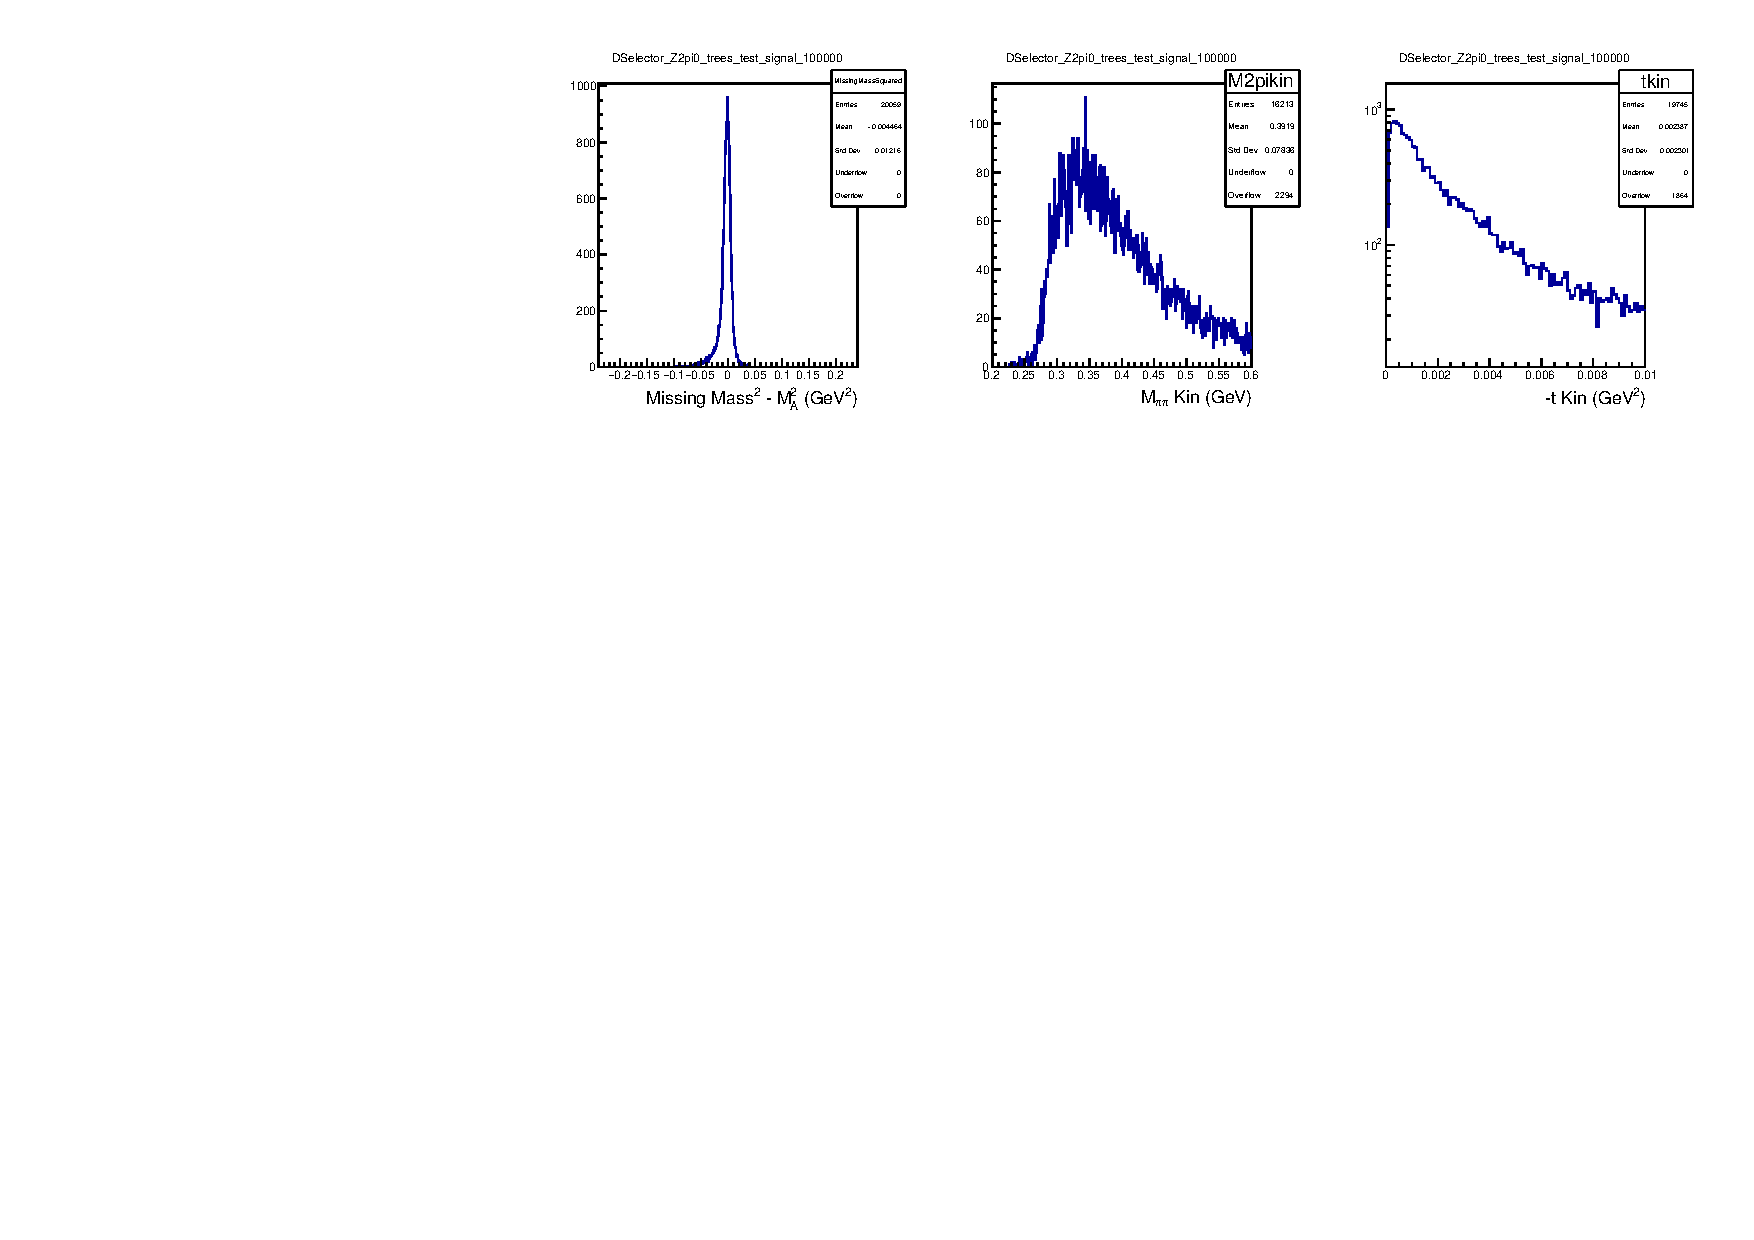
\includegraphics[width=6in]{figures/MMMpipit_signal_DSelector.pdf}
\caption{Left: Missing mass distribution minus the mass of the recoil nucleus. Center: Kinematically fit $2\pi$ mass distribution. Right: Kinematically fit $-t$ distribution.
\label{fig:MMMpipit_signal_DSelector}}
\end{figure}
The reconstructed momentum relative to its generated value is shown in
Fig.~\ref{fig:DeltapDeltaPhi_signal_DSelector}. The central peak of the
kinematically fit momentum is about 2\%, similar to that for charged
pions. However, there are long tails that will effect the
final reconstruction. The resolution of the azimuthal angle,
$\phi_{\pi\pi}$, between the production and the photon polarization
planes is quite poor owing to the fact that the pion pairs are
produced at very shallow angles. Nevertheless it is sufficient to
measure the asymmetry due to the photon beam polarization.
\begin{figure}[tph]
\centering
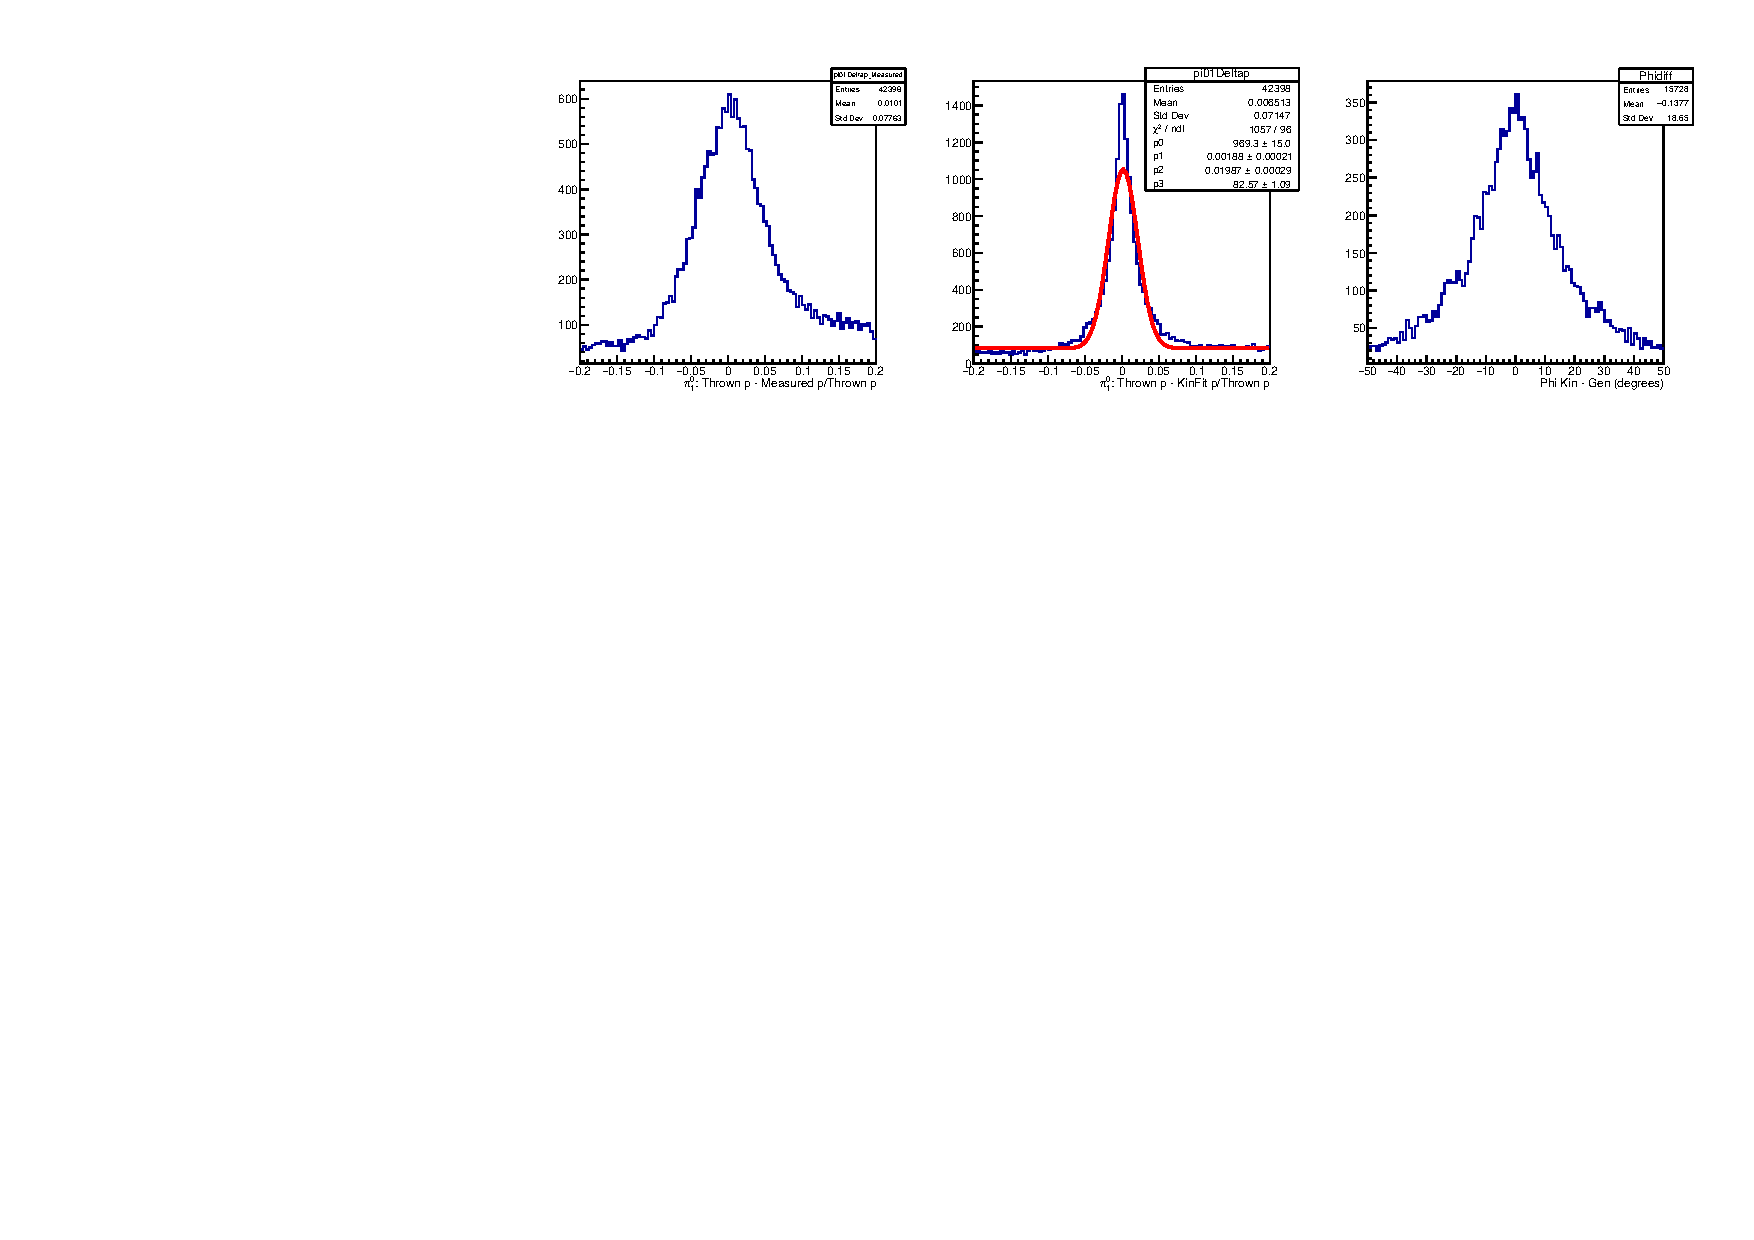
\includegraphics[width=6in]{figures/DeltapDeltaPhi_signal_DSelector.pdf}
\caption{Left: Difference between measured and generated momentum. Center: Difference between kinematically fit and generated momentum. The central peak has a width of about 2\%. Right: Difference between the kinematically fit azimuthal angle $\phi_{\pi\pi}$ and its generated value.
\label{fig:DeltapDeltaPhi_signal_DSelector}}
\end{figure}
The resolution of the 2$\pi$ invariant mass is shown in Fig.~\ref{fig:Resolution_Mpipittag_signal_DSelector}, along with the resolution of Mandelstam $-t$, and the reconstructed time resolution. The mass resolution is about 12~MeV.
\begin{figure}[tph]
\centering
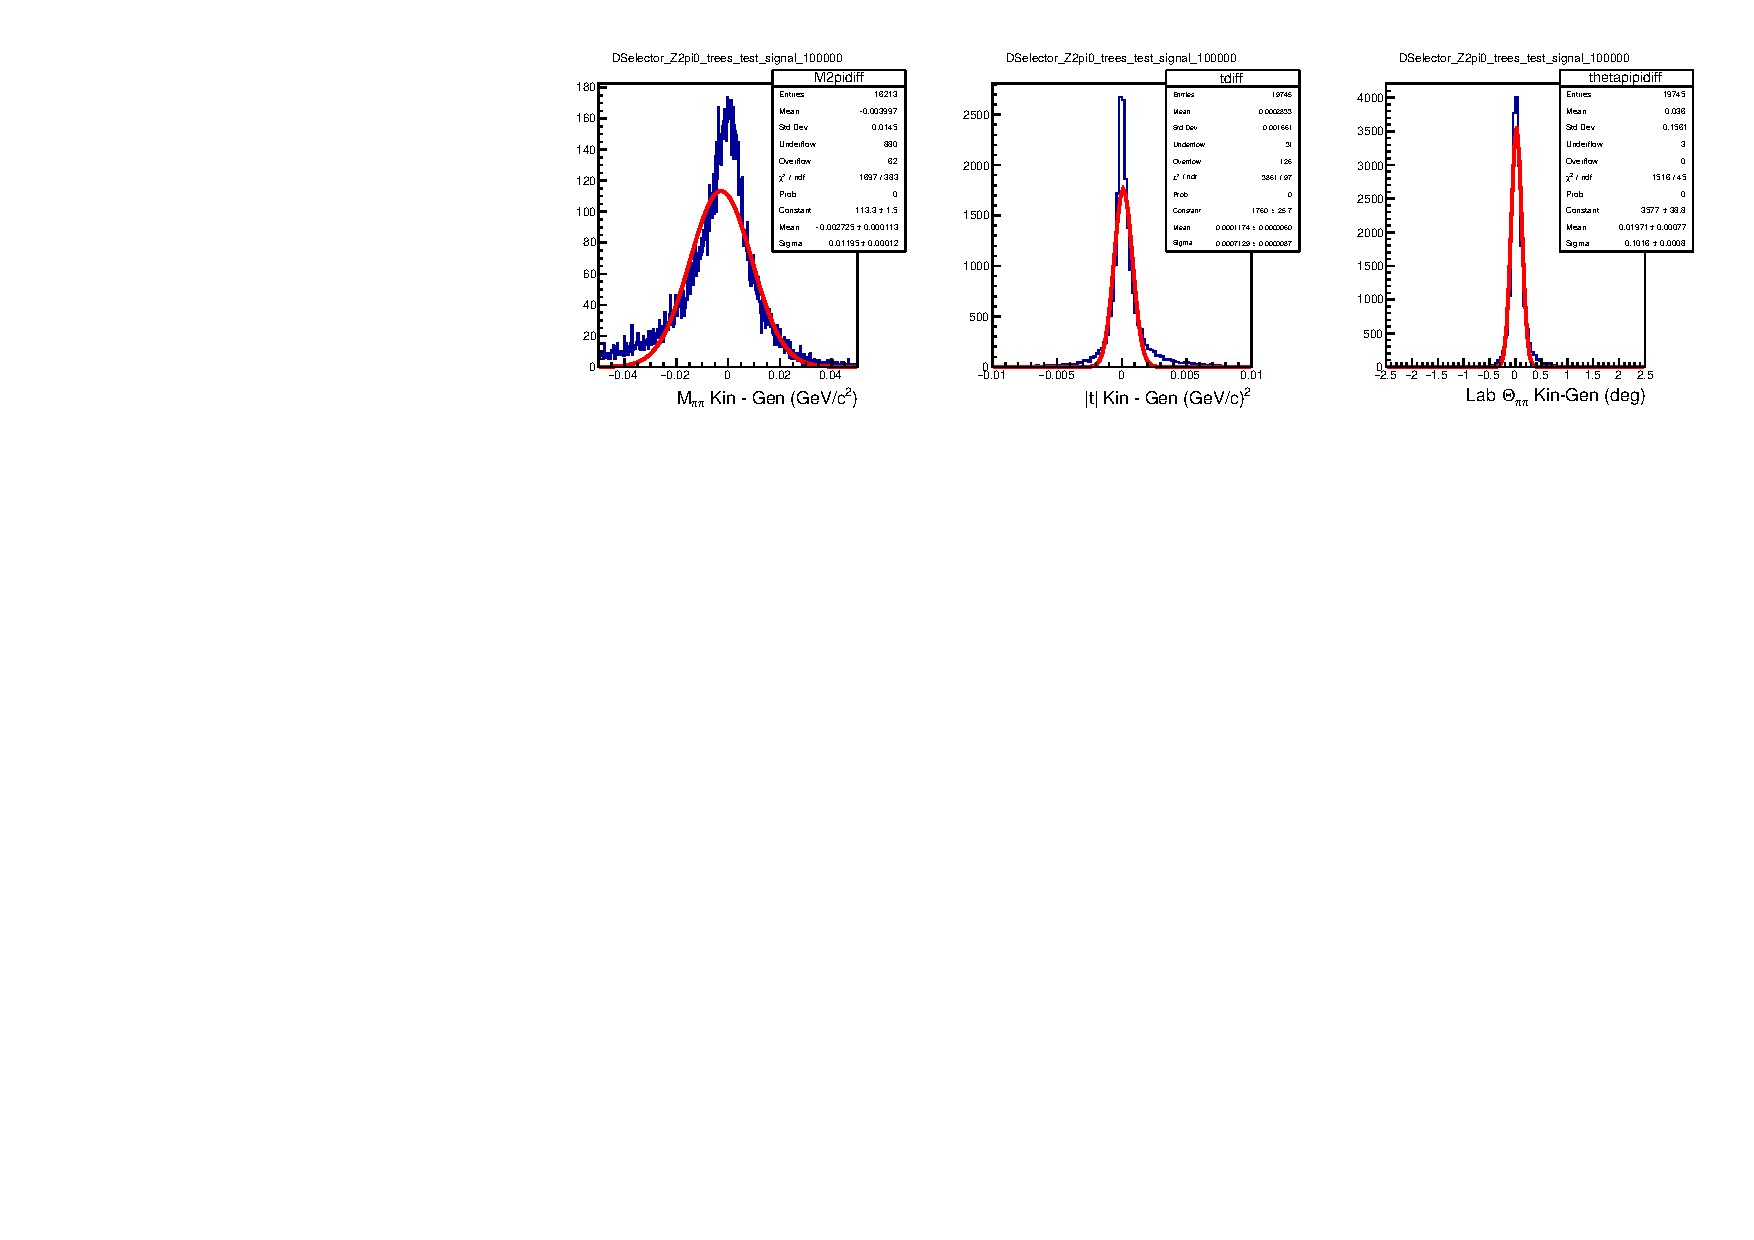
\includegraphics[width=6in]{figures/Resolution_Mpipittag_signal_DSelector.pdf}
\caption{Left: Difference between kinematically fit and generated 2$\pi$ mass. The central 2$\pi$-mass $\sigma$ is about 12 MeV. Center: Difference between kinematically fit and generated -t. Right: Difference between kinematically fit and generated 2$\pi$ polar angle. The resolution $\sigma$ of the reconstructed angle is 0.1 degrees.
%Right: Timing resolution relative to the accelerator RF signal is about 0.35 ns.
\label{fig:Resolution_Mpipittag_signal_DSelector}}
\end{figure}

\subsection{Trigger and acceptance}
The Primakoff reaction will transfer all the energy of the beam into
four photons, which are going forward. All this energy will be
deposited in the FCAL, except for leakage down the beampipe. We expect
a simple trigger with an energy threshold in the FCAL should have very
high efficiency for any events that can be reconstructed:
the FCAL trigger with the total energy threshold around 1$\,$GeV can be used. To estimate trigger rate we used the same method as for TOF trigger rate \cite{TOFrate} extracted from the dedicated runs with high random trigger frequency. We used FCAL total energy greater than 1GeV deposited within 40$\,$ns excluding the most inner FCAL layer as a trigger condition. Fig.~\ref{fig:fcalrate} shows the values for LH2 and ``empty'' target configurations.
Since the proposed lead target is 1.7 times thicker than LH2 target (in rad. lengths), we used ``empty'' target rate plus the difference between LH2 and ``empty'' target rates scaled with the factor of 1.7. That gives the value $\sim$9$\,$kHz for 20$\,$nA beam current.

\begin{figure}[tph]
\centering
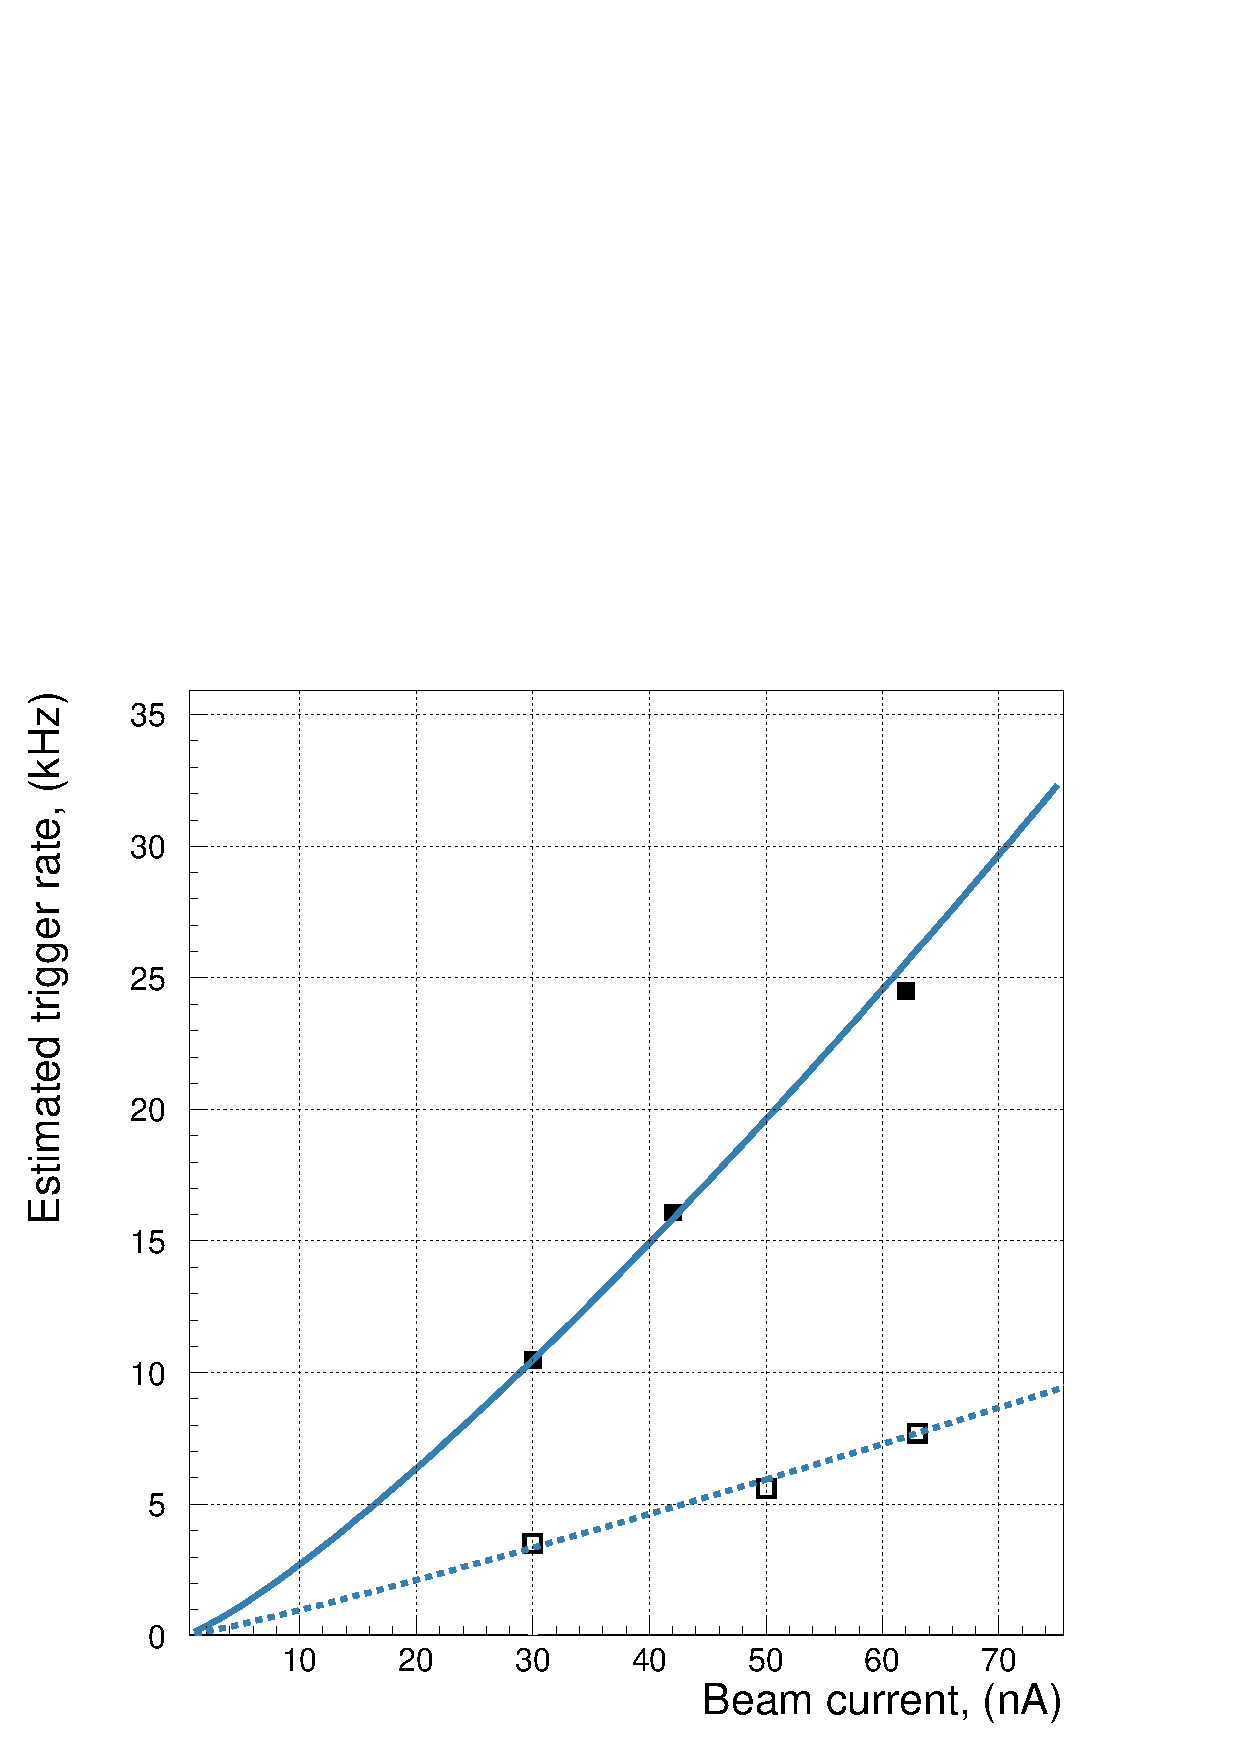
\includegraphics[width=3in]{figures/fcalrate_vs_beam.pdf}
\caption{Estimated FCAL trigger rate for 1$\,$GeV
total energy threshold for LH2 (solid squares) and ``empty'' (empty squares) targets.
\label{fig:fcalrate}}
\end{figure}

The acceptance of the signal events can be determined by comparing the
kinematically fit to the generated distributions. The generated and
kinematically fit 2$\pi$ mass, $\phi_{\pi\pi}$ and $-t$ distributions
are shown in
Fig.\,\ref{fig:twopi_primakoff_DSelect_p1_W_100000_sum}. The
reconstruction was described in the previous section.
\begin{figure}[tph]
\centering
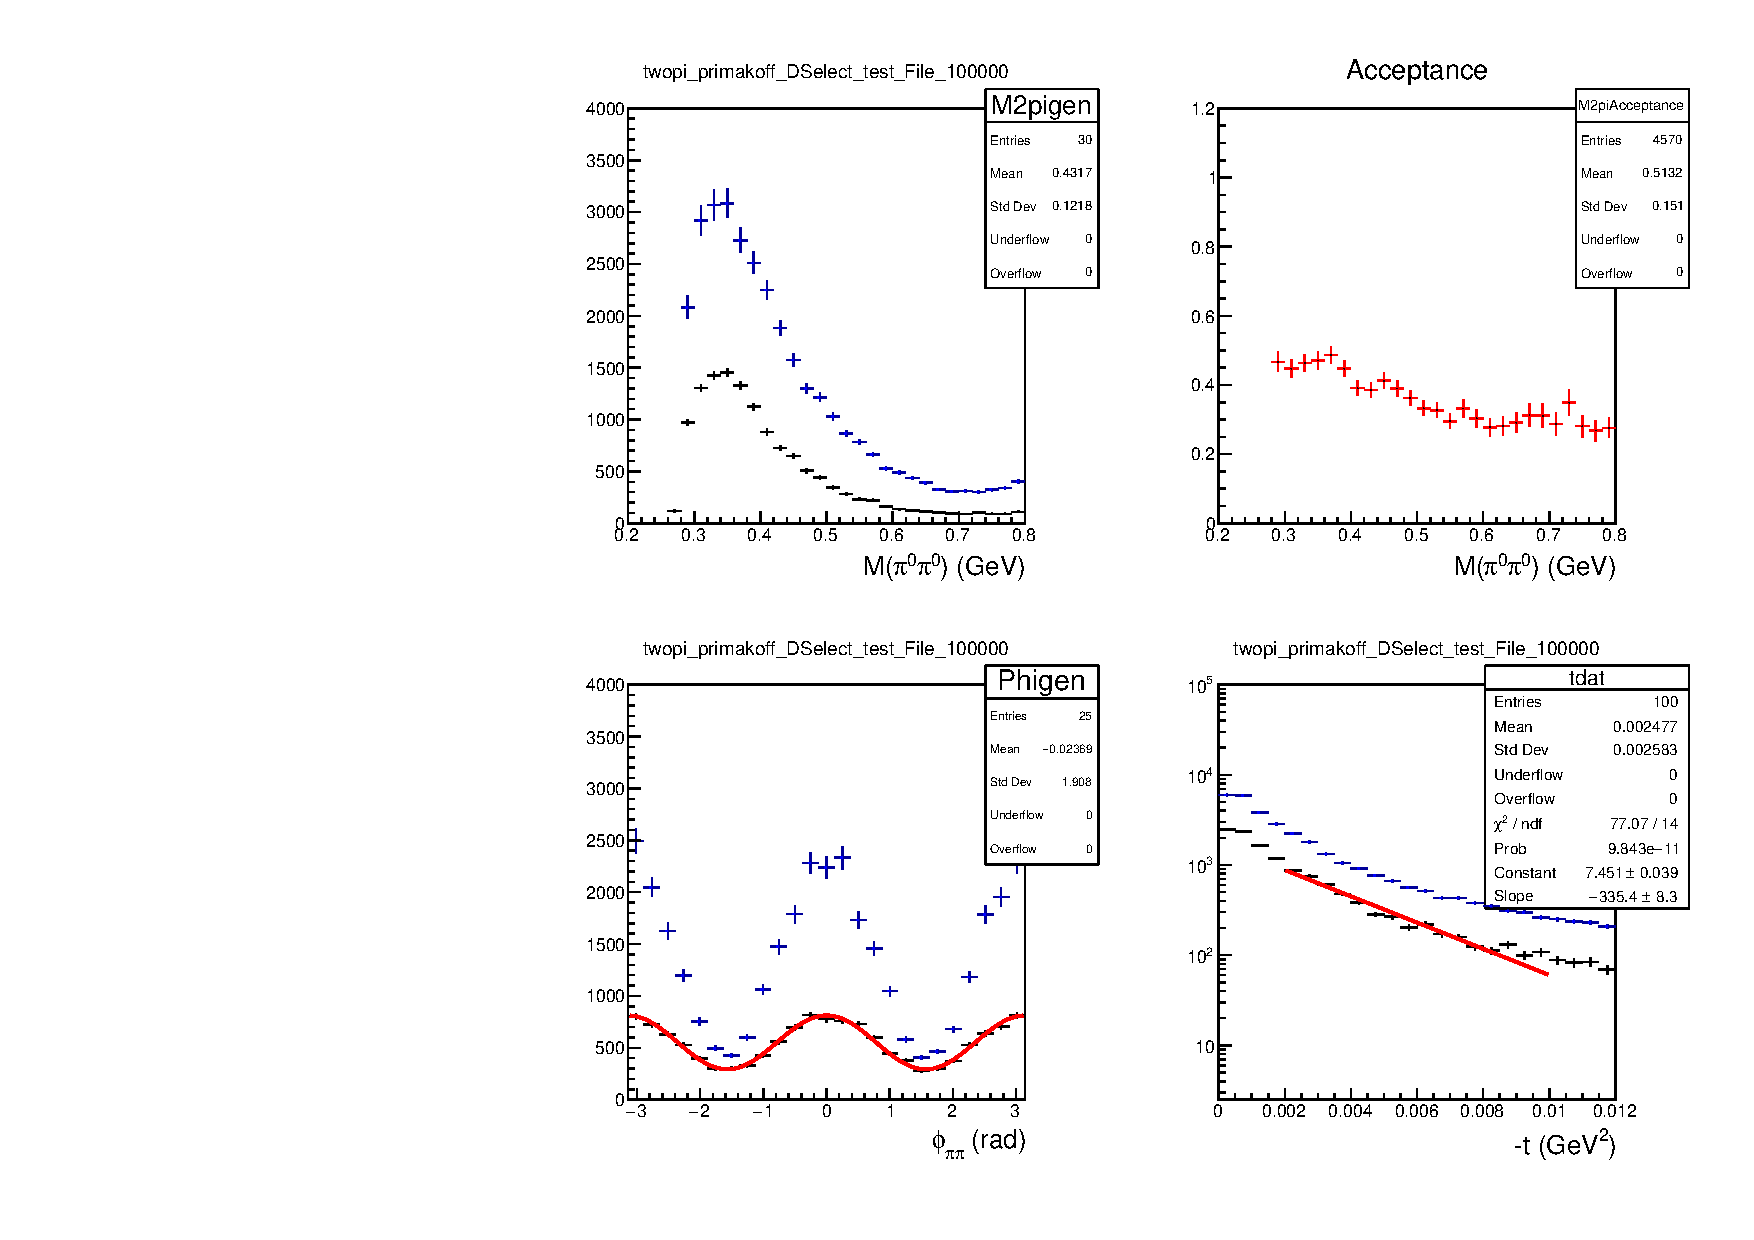
\includegraphics[width=6in]{figures/twopi_primakoff_DSelect_test_File_100000_sum_PrimNC.pdf}
\caption{Top left: Generated and kinematically fit (accepted) 2$\pi$-mass distribution. Top right: Acceptance as a function of 2$\pi$ mass. The acceptance is about 40\% at threshold. Bottom left: Generated and kinematically fit azimuthal angle $\phi_{\pi\pi}$. Bottom right: Generated and kinematically fit $-t$ distribution. }
\label{fig:twopi_primakoff_DSelect_p1_W_100000_sum}
\end{figure}
The acceptance is quite high at about 40\%. However, there is also
significant slewing due to resolution in most variables of
interest.  The
relatively poor resolution in $\phi_{\pi\pi}$ results in dilution of
the measured azimuthal dependence, which will need to be adjusted
based on simulation. Finally the measured $-t$ resolution roughly reproduces the generated slope despite the smearing of high rate regions down to low rate
regions.
